\documentclass[12pt]{article}
\usepackage{amsmath}
\usepackage{amssymb}
\usepackage{amsthm}
\usepackage{amsfonts}
\usepackage{algpseudocode}
\usepackage{algorithm}
\usepackage{mathrsfs}
\usepackage{graphicx}
\usepackage{times}
\usepackage{color}
\usepackage{appendix}
\usepackage{subfigure}
\usepackage{enumerate}
\usepackage{mathtools}
\usepackage{multirow}
\usepackage{booktabs}
\numberwithin{table}{section}
\usepackage{enumitem} %change list depth

\usepackage{listings}
\usepackage{xcolor}

\definecolor{codegreen}{rgb}{0,0.6,0}
\definecolor{codegray}{rgb}{0.5,0.5,0.5}
\definecolor{codepurple}{rgb}{0.58,0,0.82}
\definecolor{backcolour}{rgb}{0.95,0.95,0.92}

\lstdefinestyle{mystyle}{
	backgroundcolor=\color{backcolour},   
	commentstyle=\color{codegreen},
	keywordstyle=\color{magenta},
	numberstyle=\tiny\color{codegray},
	stringstyle=\color{codepurple},
	basicstyle=\ttfamily\footnotesize,
	breakatwhitespace=false,         
	breaklines=true,                 
	captionpos=b,                    
	keepspaces=true,                 
	numbers=left,                    
	numbersep=5pt,                  
	showspaces=false,                
	showstringspaces=false,
	showtabs=false,                  
	tabsize=2
}

\lstset{style=mystyle}

\usepackage{tikz}
\usetikzlibrary{positioning}
\usetikzlibrary{arrows,arrows.meta}
\setlistdepth{8}
\renewlist{itemize}{itemize}{8}

\newcommand{\question}[2][]{\begin{flushleft}
		\Large\textbf{Question #1}: \large\textit{#2}
		
\end{flushleft}}
\newcommand{\sol}{\textbf{Solution}:} %Use if you want a boldface solution line
\newcommand{\maketitletwo}[2][]{\begin{center}
		\Large{\textbf{Homework #1}
			
			ECE 590: Towards More Reliable Software} % Name of course here
		\vspace{5pt}
		
		\normalsize{Jeff Fan  \hspace{1em} $\left|\right|$ \hspace{1em}zf70@duke.edu  % Your name here
			
			\today}        % Change to due date if preferred
		\vspace{15pt}
		
\end{center}}

\begin{document}
	\maketitletwo[2]  % Optional argument is assignment number
	%Keep a blank space between maketitletwo and \question[1]
	
	\section*{Question 1: } 
	
	\textbf{a. Describe the faults classification in the papers (Drawing a graph may make  it clearer).}
	
	\textbf{Bohrbugs:} These are straightforward, solid faults that manifest consistently under a well-defined set of conditions. They are typically easier to detect and fix.
	
	\textbf{Mandelbugs:} These faults are characterized by complexity and obscurity, making their behavior appear chaotic or non-deterministic. They are influenced by interactions within the software system or its environment and may have a delayed failure occurrence.
	
	\textbf{Heisenbugs:} These are a subtype of Mandelbugs and refer to faults that change behavior or disappear when an attempt is made to probe or isolate them. Heisenbugs are known for their elusive nature; they often change behavior or disappear under investigation, like when using a debugger. This behavior can be influenced by changes in timing, memory state, or interactions with other processes.
	
	\textbf{Aging-Related Bugs:} These are also a subtype of Mandelbugs. They lead to the accumulation of errors over time in the application or its environment, resulting in increased failure rates or degraded performance. Aging-Related Bugs typically emerge over time due to the degradation of system state, resource leaks, data corruption, or accumulation of errors. These bugs become more prevalent or noticeable as the system continues to operate.
	
	In some cases, an Aging-Related Bug might exhibit characteristics of a Heisenbug. For example, a memory leak (an Aging-Related Bug) might only cause noticeable issues under certain conditions, such as when the system is under heavy load or has been running for an extended period. 
	
	And I draw a graph to illustrate their relationship.\\
	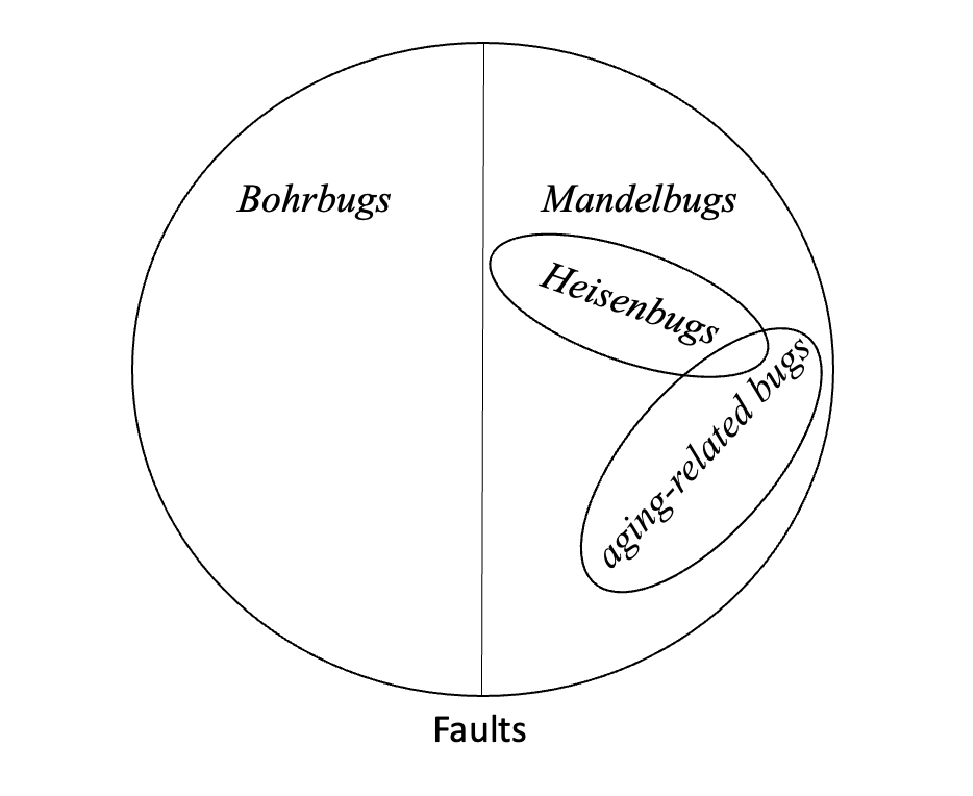
\includegraphics[width=0.7\textwidth]{1.eps}
	
	Fig. 1. The relationship of faults.\\
	\\
	\textbf{b. Explain different ways to deal with different types of bugs and to recover from the failures caused by the bugs. }
	
	\textbf{Bohrbugs:} Bohrbugs are straightforward and consistently reproducible, making them relatively easier to manage. The primary strategy is to remove them, which involves detection, diagnosis, and correction during the development and testing phases. Systematic testing, like unit and system tests, is crucial here. Early detection and removal are cost-effective and prevent these predictable bugs from affecting the operational phase.
	
	\textbf{Mandelbugs:}  Mandelbugs are complex and may not manifest consistently, making them challenging to handle. 'Retry' and 'Replicate' are effective. 'Retry' involves re-executing the failed action, which might succeed due to the non-deterministic nature of these bugs. 'Replication' uses redundant resources or systems to take over if a failure occurs. These methods are used because Mandelbugs' behavior is often unpredictable, and traditional debugging methods might not be feasible.
	
	\textbf{Heisenbugs:} Heisenbugs change behavior when investigated, making them elusive. Similar to Mandelbugs, strategies like retrying actions or replicating processes are useful. It's like trying to locate a noise in your car that stops whenever you take it to the mechanic. Keeping a log of when it happens could help identify patterns. Additionally, detailed logging and monitoring can help capture their state and behavior before they alter. These bugs require such approaches because traditional debugging might cause them to disappear or behave differently.
	
	\textbf{Aging-Related Bugs:} These bugs emerge over time, leading to gradual system degradation. The key strategy is 'Rejuvenation', which includes proactive measures like restarting systems or components before failures occur. Think of an old computer that slows down over time. Regularly rebooting it (rejuvenation) can help maintain its performance. This can be done based on monitoring system performance and identifying signs of aging. This approach is effective because it prevents the accumulation of errors or resource depletion that typically cause aging-related issues.
	
			
		\end{document}
